\begin{blocksection}
\question (Reverse Environment Diagram) Fill in each blank in the code example below so that its environment diagram matches the image. 
You should make your answers for each part as simple as possible. There may be more than one correct answer.
\newline
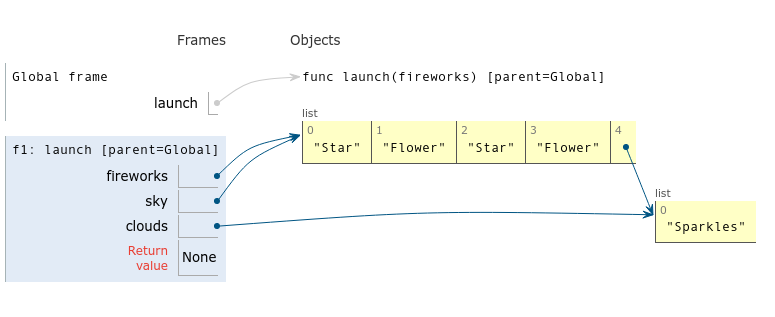
\includegraphics[width=.9\textwidth]{fireworks-diagram.png}
\newline

\begin{lstlisting}
def launch(fireworks):
    sky = fireworks
    sky.extend(____1____)
    fireworks.append(____2____)
    clouds = ____3____

launch(["Star", "Flower"])
\end{lstlisting}
\end{blocksection}

\begin{blocksection}
\begin{parts}
\part
Write an expression that could complete blank 1.
\begin{solution}[1in]
\begin{lstlisting}
fireworks OR sky
\end{lstlisting}
\end{solution}

\part
Write an expression that could complete blank 2.
\begin{solution}[1in]
\begin{lstlisting}
["Sparkles"]
\end{lstlisting}
\end{solution}

\part
Write an expression that could complete blank 3.
\begin{solution}[1in]
\begin{lstlisting}
fireworks[4] OR sky[4]
\end{lstlisting}
\end{solution}
\end{parts}
\end{blocksection}

\begin{guide}
    \begin{blocksection}
    \textbf{Teaching Tips}
    
    \begin{itemize}
    \item The purpose of this problem is to give an example of how list mutation might look like in environment diagrams. 
    Since the previous questions on the worksheet already cover mutation, you can emphasize how even though the reverse ED format may feel unfamiliar, 
    the content is really the same as what they've been doing for the past section.
    \item A good way to introduce the problem is to share some of your own tips and thought processes on how to tackle reverse environment diagrams 
    (matching data types, running it through pythontutor, starting with placeholder values...) so your students have a sense of direction moving into the problem.
    \item Make sure to explain the difference between \lstinline{append} and \lstinline{extend}! Students often get these mixed up.
    \item If you choose to walk through the problem on pythontutor, make sure you use tutor.cs61a.org and NOT pythontutor.org, since the former has all of the formatting
          rules set up (frame numbers, parents, etc)
    \item Alex's Guide to Reverse Environment Diagrams:
        \begin{itemize}
            \item Fill in the blanks with random/default/generic values.
            \item Run through the code line by line to construct your own environment diagram.
            \item If your environment diagram doesn't match the image, go back to step 1 and try to fix each blank one by one.
        \end{itemize}
    \end{itemize}
    \end{blocksection}
    \end{guide}